\section{Lucenarium}

\opis{Potrzebne: 6(4) ministrantów siedzących w chórze, \cc2 lub \tt~ (gdy nie
	ma \cc2 \tt~ prowadzi i daje znaki), 6(4) pochodni wystawionych koło bazy \tt}

\begin{itemize}
	\item Po okadzeniu ludu \tt~ zatrzymuje się n przy stopniu prezbiterium i
	      zwraca się w kierunku ołtarza. Dołącza do niego \cc2 i 6 ministrantów
	      wyznaczonych do lucenarium.
	\item Na znak \cc2 klękają i wychodzą do bocznej nawy po pochodnie.	(Rys.
	      \ref{fig:wyjscie})
	\item Przygotowują pochodnie, mogą zasypać kadzielnicę.
	\item Na śpiew \textit{Sanctus} bardzo powoli wchodzą do prezbiterium
	      rozchodząc się na boki (Rys.\ref{fig:wejscie_1})
	\item Ustawieni odpowiednio przyklękają, po czym klękają na dwa kolana
	      (Rys.\ref{fig:wejscie_2})
	\item \tt~ zajmuje miejsce z prawej strony na pierwszym stopniu ołtarza.
	      Klęczą przez cały Kanon.
	\item Na \textit{Per omnia saecula saeculorum} wstają, wykonują skłon na
	      \textit{Oremus}, a następnie przyklękają i na czele z \tt~ i \cc2
	      wychodzą z prezbiterium (Rys. \ref{fig:wyjscie_1} oraz Rys.
	      \ref{fig:wyjscie_2})
\end{itemize}

\begin{figure}[h]
	\centering
	\includegraphics[width=0.29\linewidth]{wyjscie}
	\caption{Wyjście ministrantów podczas ofiarowania}
	\label{fig:wyjscie}
\end{figure}

\begin{figure}[ht]
	\savebox{\imagebox}{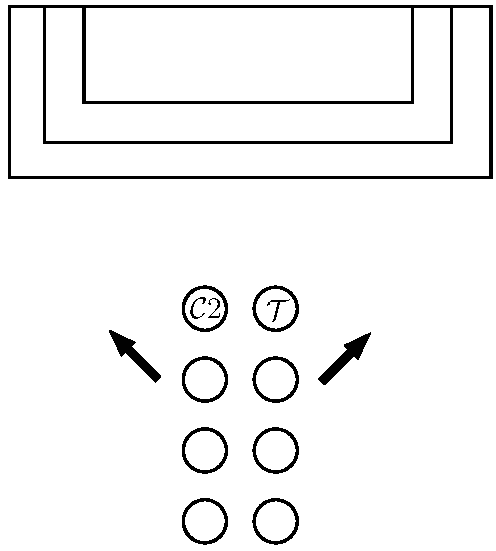
\includegraphics[width=.4\linewidth]{wejscie_1}}%
	\begin{subfigure}[t]{.5\linewidth}
		\centering\usebox{\imagebox}
		\caption{Przed przyklęknięciem}
		\label{fig:wejscie_1}
	\end{subfigure}\qquad
	\begin{subfigure}[t]{.5\linewidth}
		\centering\raisebox{\dimexpr\ht\imagebox-\height}{% Raise smaller image
			into place \includegraphics[width=\linewidth]{wejscie_2}}%
		\caption{Po przyklęknięciu}
		\label{fig:wejscie_2}
	\end{subfigure}
	\caption{Wejście ministrantów na \textit{Sanctus}}
\end{figure}

\newpage

\begin{figure}[ht]
	\savebox{\imagebox}{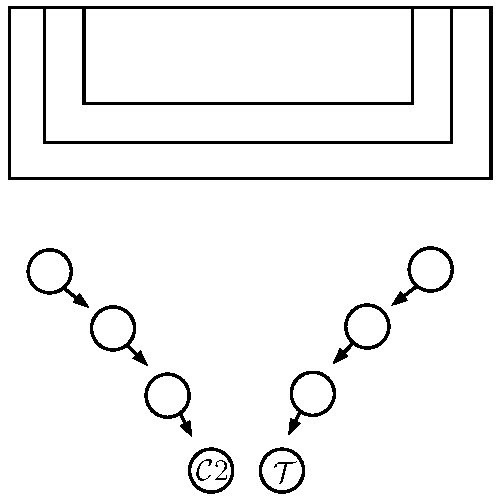
\includegraphics[width=.4\linewidth]{wyjscie_2}}%
	\begin{subfigure}[t]{.5\linewidth}
		\centering\raisebox{\dimexpr\ht\imagebox-\height}{% Raise smaller image
			into place 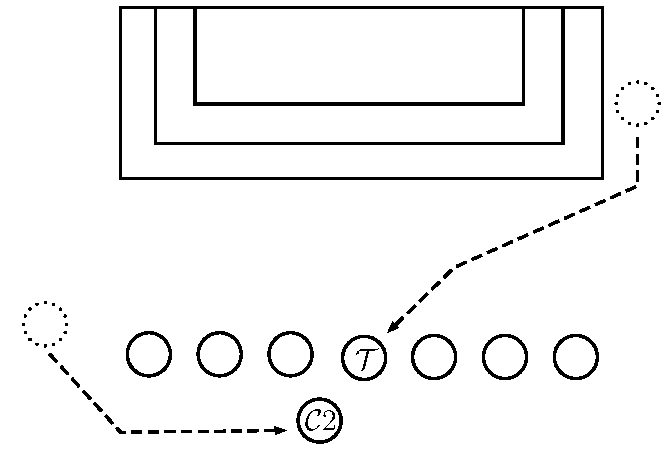
\includegraphics[width=\linewidth]{wyjscie_1}}%
		\caption{Przed przyklęknięciem}
		\label{fig:wyjscie_1}
	\end{subfigure}\qquad
	\begin{subfigure}[t]{.5\linewidth}
		\centering\usebox{\imagebox}
		\caption{Po przyklęknięciu}
		\label{fig:wyjscie_2}
	\end{subfigure}
	\caption{Wyjście ministrantów po \textit{Per omnia secula seculorum}}
\end{figure}

\textbf{Uwaga!} Na Mszy Wieczerzy Pańskiej w Wielki Czwartek ministranci z
pochodniami nie wychodzą z prezbiterium, tylko oczekują na procesję.